\chapter{Диаграммы Пенроуза и образование реальной чёрной дыры}

Картина Крускала даёт изящное описание окрестности горизонта Шварцшильда, но реальная чёрная дыра не вечна: она образуется при коллапсе вещества. Какие части этой расширенной картины переживают такую физическую историю? Чтобы ответить на этот вопрос, нам нужна диаграмма, достаточно большая, чтобы вместить всё пространство-время, и достаточно строгая, чтобы сохранять ход световых лучей. Сначала мы выполним компактификацию плоского пространства-времени, затем — пространства-времени Шварцшильда, а в конце сошьём подходящие части через падающую внутрь оболочку излучения.

\section{Вблизи горизонта: краткое повторение Крускала и четыре квадранта}

Начнём в точности с того места, на котором закончилась предыдущая лекция. Совсем близко к горизонту Шварцшильда геометрия локально выглядит как плоское пространство. Сам горизонт в полярных координатах ведёт себя как гиперболическое геометрическое место точек, подобно тому как это происходит для ускоренных координат в обычном пространстве-времени Минковского. В этой локальной картине мы с самого начала вводим одно правило и больше его не ослабляем: радиальные световые лучи изображаются под углом \(45^\circ\), и любая времениподобная мировая линия должна оставаться круче этих нулевых линий.

Координаты в этом повторении лучше всего понимать как время и пространство в описании свободно падающего наблюдателя. В этих локально инерциальных координатах окрестность горизонта выглядит почти плоской. Но наблюдатель, который настаивает на том, чтобы висеть с фиксированным радиусом вне дыры, не является инерциальным. Относительно свободно падающей системы отсчёта такой человек описывает ускоренную кривую. Чем ближе он висит к горизонту, тем большее ускорение нужно, чтобы удержаться снаружи. Именно в этом состоит физический смысл семейства внешних кривых, нарисованных в правой части доски.

\begin{figure}[htbp]
\centering
\includegraphics[width=0.72\textwidth]{lecture_08_figure_02.png}
\caption{Эскиз на доске геометрии вблизи горизонта с четырьмя областями. Красные кривые во внешней области показывают семейство мировых линий наблюдателей, зависающих на фиксированном радиусе.}
\lectureframe{00:02:54}
\end{figure}

\begin{figure}[htbp]
\centering
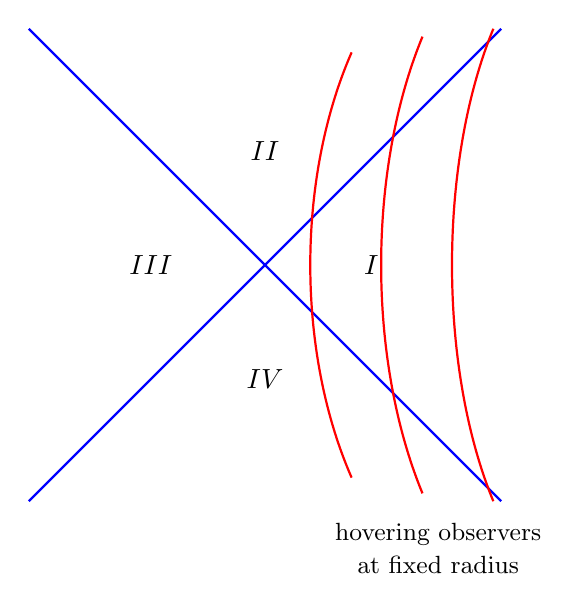
\begin{tikzpicture}[scale=1.0]
\draw[thick,blue] (-3,3) -- (3,-3);
\draw[thick,blue] (-3,-3) -- (3,3);

\draw[red,thick] (1.1,-2.7) .. controls (0.4,-1.1) and (0.4,1.1) .. (1.1,2.7);
\draw[red,thick] (2.0,-2.9) .. controls (1.3,-1.2) and (1.3,1.2) .. (2.0,2.9);
\draw[red,thick] (2.9,-3.0) .. controls (2.2,-1.3) and (2.2,1.3) .. (2.9,3.0);

\node at (1.35,0.0) {$I$};
\node at (0.0,1.45) {$II$};
\node at (-1.45,0.0) {$III$};
\node at (0.0,-1.45) {$IV$};

\node[align=center] at (2.2,-3.6) {\small hovering observers\\\small at fixed radius};
\end{tikzpicture}
\caption{Аккуратная перерисовка причинной структуры в стиле Крускала, использованной в этом повторении. Область \(I\) — внешняя, область \(II\) — внутренняя область без выхода, а области \(III\) и \(IV\) принадлежат формальному продолжению, которое позднее будет отброшено для реальной коллапсирующей чёрной дыры.}
\end{figure}

Этого уже достаточно, чтобы сказать, что делает чёрная дыра. Во внешней области \(I\) объекты и сигналы могут идти внутрь, но могут также оставаться снаружи или повернуть обратно наружу. В области \(II\), напротив, каузальный вывод уже фиксирован. Оказавшись внутри, нельзя вернуться наружу ни по какому будущенаправленному причинному пути. Чтобы выбраться из области \(II\) в любую из внешних областей, потребовалась бы траектория, которая где-то была бы более пологой, чем \(45^\circ\), а значит, быстрее света. Любая допустимая будущенаправленная времениподобная траектория заканчивается на сингулярности.

Это вводное повторение — не просто повторение. Оно подготавливает главную тему главы. Картина Крускала полезна, но не вся она физически осмысленна для реальной чёрной дыры.

\begin{classroomqa}
\audiencequestion{Каковы оси диаграммы и чьи мировые линии с фиксированным положением образуют красные кривые?}
\lecturerresponse{Это время и пространство в координатах, естественных для свободно падающего наблюдателя. Вблизи горизонта он видит почти обычное плоское пространство-время. Красные же кривые постоянного положения принадлежат наблюдателям, которых удерживают неподвижными вне дыры. Это ускоренные мировые линии, причём требуемое ускорение возрастает по мере приближения к горизонту.
\lecturetimestamp{00:05:58--00:06:47}}
\end{classroomqa}

\section{Зачем нужна компактификация? От бесконечного пространства-времени к конечному рисунку на доске}

Следующий шаг носит методологический характер. Нулевые направления на этих диаграммах уходят в бесконечность, и туда же уходит само время. Поэтому мы не можем изобразить всё пространство-время на обычной доске, если не сменим координаты. Мотивация лектора весьма конкретна: если мы хотим увидеть всё сразу и рассуждать о глобальной причинной структуре, нам нужен способ сжать бесконечное пространство-время в конечную область, сохранив световые лучи узнаваемыми.

Поэтому он отступает к простому случаю — к старому доброму плоскому пространству-времени. Поскольку интересующие нас задачи сферически симметричны, мы опускаем угловые направления и оставляем только время и радиальную координату. Мы используем координаты \(T\) и \(R\), причём
\[
R\ge 0,
\]
поскольку отрицательное радиальное расстояние в полярных координатах не имеет смысла. Мы также выбираем единицы, в которых
\[
c=1.
\]
При этом соглашении радиальное нулевое движение изображается под углом \(45^\circ\).

Прежде чем ввести компактифицирующее отображение, лекция уделяет некоторое время тому, чтобы сориентировать нас в плоскости \(T\)-\(R\). Рисуют ось времени, радиальную ось, несколько срезов постоянного времени \(T=0,\pm1,\pm2\) и несколько линий постоянного радиуса \(R=1,2,3\). Это не пустой формализм. Он даёт нам ориентиры и проясняет, какие именно черты мы хотим сохранить, когда позднее диаграмма будет сжата до конечного размера.

Здесь есть и тонкий, но важный педагогический момент, связанный с началом координат. В редуцированной радиальной картине световой луч, направленный точно в \(R=0\), выглядит так, будто он отскакивает от начала координат и снова выходит наружу. Но физически ничто не отражается ни от какой стенки. В полной сферически-симметричной геометрии луч просто проходит через начало координат и выходит с другой стороны. Кажущийся отскок — лишь следствие того, что мы работаем с полуплоскостью \(R\ge 0\).

Точно так же световой луч, не попадающий в начало координат, сначала выглядит почти так же, достигает точки наибольшего сближения, а затем поворачивает обратно наружу. В этих координатах может даже показаться, будто что-то оттолкнуло его от начала координат. Но и это — лишь координатное описание привычного барьера углового момента, а не новой силы. Лектор задерживается на этих примерах, потому что хочет, чтобы аудитория доверяла диаграмме ещё до того, как он начнёт её деформировать.

Теперь начинается главный ход. Мы собираемся сжимать и растягивать картину, но сохраним неизменным одно: радиальные световые лучи должны оставаться линиями под углом \(45^\circ\). В этом и состоит весь смысл компактификации.

\begin{classroomqa}
\audiencequestion{Есть ли что-нибудь физически особенное в выбранном начале координат и свидетельствуют ли кажущиеся искривлённые лучи о наличии там силы?}
\lecturerresponse{Нет. На этом этапе начало координат — всего лишь центр, выбранный сферическими координатами. Кажущиеся отскок и изгиб возникают из-за сведения полного пространственного движения к \(R\geq0\). Симметрия может делать центр удобным, как в случае Солнца, но выбор координат не помещает туда чёрную дыру или отражающую стенку.
\lecturetimestamp{00:16:27--00:17:08}}
\end{classroomqa}

\section{Плоское пространство-время в нулевых координатах и в форме Пенроуза}

Чтобы сделать эту деформацию точной, мы вводим нулевые координаты. Это математически аккуратная часть лекции, и на доске этот шаг выписан явно.

\begin{figure}[htbp]
\centering
\includegraphics[width=0.82\textwidth]{lecture_08_figure_03.png}
\caption{Незагромождённая доска в плоскости \(T\)-\(R\) при введении
\(T^+=T+R\) и \(T^-=T-R\). Редуцированное радиальное начало — это синяя вертикальная линия
\(R=0\).}
\lectureframe{00:19:45}
\end{figure}

Мы определяем
\begin{align}
T^+ &= T+R, \\
T^- &= T-R.
\end{align}
Они приспособлены к радиальному нулевому движению. Для входящего радиального светового луча имеем \(T^+=\text{const}\), тогда как для исходящего радиального светового луча имеем \(T^-=\text{const}\).

\paragraph{Подробный вывод.}
Линия \(R=0\) в этих координатах становится особенно простой. В самом деле,
\begin{align}
R=0
&\iff T+R=T-R \\
&\iff T^+=T^-.
\end{align}
Итак, вся времениподобная граница \(R=0\) описывается единственным соотношением
\begin{equation}
R=0 \iff T^+=T^-.
\end{equation}

\begin{figure}[htbp]
\centering
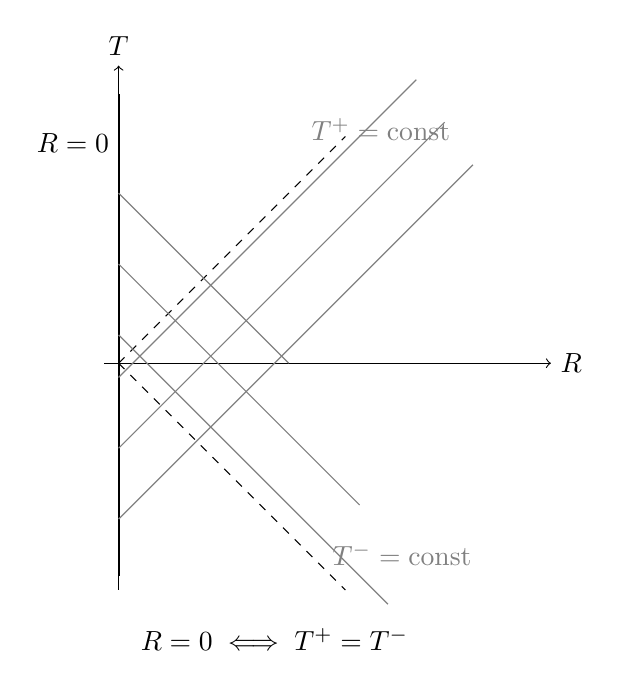
\begin{tikzpicture}[scale=0.9]
\draw[->] (-0.2,0) -- (6.1,0) node[right] {$R$};
\draw[->] (0,-3.2) -- (0,4.2) node[above] {$T$};

\draw[thick] (0,-3.0) -- (0,3.8);
\node[left] at (0,3.1) {$R=0$};

\draw[dashed] (0,0) -- (3.2,3.2);
\draw[dashed] (0,0) -- (3.2,-3.2);

\draw[gray] (0,2.4) -- (2.4,0);
\draw[gray] (0,1.4) -- (3.4,-2.0);
\draw[gray] (0,0.4) -- (3.8,-3.4);

\draw[gray] (0,-2.2) -- (5.0,2.8);
\draw[gray] (0,-1.2) -- (4.6,3.4);
\draw[gray] (0,-0.2) -- (4.2,4.0);

\node[gray] at (3.7,3.3) {$T^+=\mathrm{const}$};
\node[gray] at (4.0,-2.7) {$T^-=\mathrm{const}$};

\node at (2.2,-3.9) {$R=0 \iff T^+=T^-$};
\end{tikzpicture}
\caption{Аккуратная перерисовка в плоскости \(T\)-\(R\). Два нулевых семейства задаются уровнями \(T^+\) и \(T^-\), а линия \(R=0\) эквивалентно записывается как \(T^+=T^-\).}
\end{figure}

Теперь выполняем компактификацию. Мы вводим две новые нулевые координаты \(U^\pm\), каждая из которых получается из соответствующей \(T^\pm\) одной и той же ограниченной монотонной функцией \(F\):
\begin{align}
U^+ &= F(T^+), &
U^- &= F(T^-),
\end{align}
причём
\begin{equation}
F(+\infty)=1,
\qquad
F(-\infty)=-1.
\end{equation}
В лекции для удобства выбирается
\begin{equation}
F(x)=\tanh x,
\end{equation}
так что
\begin{equation}
U^+ = \tanh(T^+),
\qquad
U^- = \tanh(T^-).
\end{equation}
Гиперболический тангенс здесь ничем не привилегирован. Это просто гладкая функция с нужным предельным поведением, и потому она сжимает бесконечные диапазоны координат до конечных.

Нулевая структура сохраняется по простой причине. Если для входящего радиального светового луча выполняется \(T^+=\text{const}\), то
\[
U^+=F(T^+)=\text{const},
\]
и аналогично, если для исходящего радиального светового луча выполняется \(T^-=\text{const}\), то
\[
U^-=F(T^-)=\text{const}.
\]
Таким образом, компактификация по отдельности перепараметризует два нулевых направления, и радиальные световые лучи остаются линиями под углом \(45^\circ\). Линия начала координат переносится столь же просто:
\[
T^+=T^- \Longrightarrow U^+=U^-.
\]

К этому моменту бесконечная полуплоскость плоского пространства-времени сжата в конечный треугольник. Затем лекция учит нас читать его границы. Пространственная бесконечность стягивается в одну точку \(i^0\). Будущая и прошлая времениподобные бесконечности — это \(i^+\) и \(i^-\). Две нулевые границы — это \(\mathcal{I}^+\) и \(\mathcal{I}^-\), их часто произносят как «скрай-плюс» и «скрай-минус»; это места, где начинаются и заканчиваются входящие и исходящие световые лучи.

\begin{figure}[htbp]
\centering
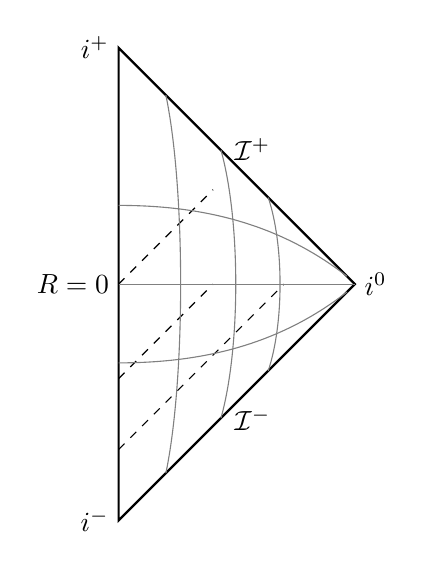
\begin{tikzpicture}[scale=1.0]
\draw[thick] (0,-3) -- (0,3) -- (3,0) -- cycle;

\node[left] at (0,3) {$i^+$};
\node[left] at (0,-3) {$i^-$};
\node[right] at (3,0) {$i^0$};
\node[left] at (0,0) {$R=0$};
\node[above right] at (1.35,1.45) {$\mathcal{I}^+$};
\node[below right] at (1.35,-1.45) {$\mathcal{I}^-$};

\draw[dashed] (0,-2.1) -- (2.1,0.0);
\draw[dashed] (0,-1.2) -- (1.2,0.0);
\draw[dashed] (0,0.0) -- (1.2,1.2);

\draw[gray] (0,0) -- (3,0);
\draw[gray] (0,1.0) .. controls (1.0,1.0) and (2.0,0.8) .. (2.9,0.1);
\draw[gray] (0,-1.0) .. controls (1.0,-1.0) and (2.0,-0.8) .. (2.9,-0.1);

\draw[gray] (0.6,-2.4) .. controls (0.85,-1.2) and (0.85,1.2) .. (0.6,2.4);
\draw[gray] (1.3,-1.7) .. controls (1.55,-0.8) and (1.55,0.8) .. (1.3,1.7);
\draw[gray] (1.9,-1.1) .. controls (2.1,-0.5) and (2.1,0.5) .. (1.9,1.1);
\end{tikzpicture}
\caption{Диаграмма Пенроуза для радиально редуцированного плоского пространства-времени. Линии постоянного времени идут наружу к \(i^0\), а линии постоянного радиуса поднимаются от \(i^-\) к \(i^+\).}
\end{figure}

Следует помнить ещё об одном замечании из лекции. Эти диаграммы \emph{не} сохраняют метрический масштаб. Они сохраняют причинную структуру. Именно этот инвариант нас и интересует.

\begin{classroomqa}
\audiencequestion{Должны ли компактифицированные линии постоянного времени быть прямыми?}
\lecturerresponse{Прямым при выбранном отображении является только симметричное сечение \(T=0\). Остальные кривые с постоянным \(T\) изгибаются, и их точная форма зависит от функции компактификации. Очень поздние сечения скапливаются всё ближе к верхней границе, хотя обычное время продолжает неограниченно возрастать.
\lecturetimestamp{00:29:11--00:30:12}}
\end{classroomqa}

\section{Компактифицированная геометрия Шварцшильда}

Используя построение для плоского пространства, мы теперь возвращаемся к чёрной дыре и повторяем ту же процедуру. Мы компактифицируем геометрию Крускала, вводя нулевые координаты и сжимая бесконечные диапазоны в конечную фигуру. Лектор описывает результат как диагональный прямоугольник или ромбовидную причинную картину: горизонт появляется как нулевая граница, мировые линии зависающих снаружи наблюдателей остаются вне него, а внутренняя область оканчивается на сингулярности, которая теперь видна на рисунке.

Решающая физическая мысль состоит в том, что для падающего наблюдателя сингулярность \emph{не} находится на бесконечности. После пересечения горизонта оставшееся собственное время до столкновения с сингулярностью конечно. Диаграмма Пенроуза делает это визуально неизбежным.

Горизонт снова задаётся условием Шварцшильда
\begin{equation}
1-\frac{2MG}{r}=0
\qquad \Longleftrightarrow \qquad
r=2MG.
\end{equation}
Равенство \(r=2MG\) отмечает радиус, на котором шварцшильдовский множитель меняет знак.

\begin{figure}[htbp]
\centering
\includegraphics[width=0.72\textwidth]{lecture_08_figure_04.png}
\caption{Эскиз на доске, противопоставляющий формальную расширенную картину физически существенной области чёрной дыры. Красная надпись \emph{сингулярность} явно присутствует на доске.}
\lectureframe{00:37:59}
\end{figure}

\begin{figure}[htbp]
\centering
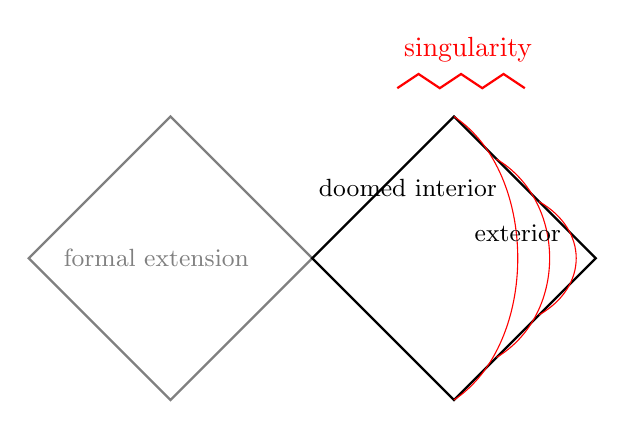
\begin{tikzpicture}[scale=0.9]
\draw[gray,thick] (-4,0) -- (-2,2) -- (0,0) -- (-2,-2) -- cycle;
\draw[thick] (0,0) -- (2,2) -- (4,0) -- (2,-2) -- cycle;

\draw[red,thick] (1.2,2.4) -- (1.5,2.6) -- (1.8,2.4) -- (2.1,2.6) -- (2.4,2.4) -- (2.7,2.6) -- (3.0,2.4);
\node[red] at (2.2,2.95) {singularity};

\draw[red] (2.0,-2.0) .. controls (3.2,-1.2) and (3.2,1.2) .. (2.0,2.0);
\draw[red] (2.6,-1.4) .. controls (3.6,-0.8) and (3.6,0.8) .. (2.6,1.4);
\draw[red] (3.2,-0.8) .. controls (3.9,-0.4) and (3.9,0.4) .. (3.2,0.8);

\node at (2.9,0.35) {\small exterior};
\node at (1.35,1.0) {\small doomed interior};
\node[gray] at (-2.2,0.0) {\small formal extension};
\end{tikzpicture}
\caption{Осторожная перерисовка причинной картины, подчёркнутой в лекции: сохранившаяся внешняя область, обречённая внутренняя область, будущая сингулярность и контраст с дополнительной формальной частью расширения.}
\end{figure}

Здесь лекция выражается предельно прямо. Если вы находитесь во внешней области, вы ещё можете уйти на бесконечность или можете упасть внутрь. Если вы находитесь во внутренней области, вы обречены. Диаграмма уже сообщает всё существенное о причинном движении, направленном в будущее.

Квадранты \(III\) и \(IV\) являются полноправными частями максимально расширенного решения Крускала. Область \(III\) даёт вторую внешнюю область, а область \(IV\) представляет собой обращённую по времени область чёрной дыры. Однако в пространстве-времени обычной чёрной дыры, образованной коллапсом, они не возникают. Расширенное решение математически поучительно именно потому, что построение коллапса покажет нам, какие части необходимо отбросить.

\section{Пространственные сечения, двумерные сферы и мост Эйнштейна--Розена}

Теперь зафиксируем компактифицированную диаграмму на пространственноподобном сечении и спросим, как это сечение выглядит как \emph{пространство}, а не как пространство-время. Именно здесь возникает образ кротовой норы, и именно здесь нельзя позволить пространственной картине забежать вперёд относительно причинного аргумента.

Поскольку угловые направления опущены, каждая точка радиальной диаграммы представляет двумерную сферу. При шварцшильдовском радиусе \(r\) её площадь равна
\begin{equation}
A=4\pi r^2.
\end{equation}
Следовательно, пространственноподобное сечение — это семейство двумерных сфер, а не просто одномерная кривая. Их размер меняется по мере движения вдоль сечения.

Вдали эти сферы очень велики. По мере продвижения внутрь их радиус уменьшается, пока не достигает минимума на горизонте,
\begin{equation}
r_{\min}=2MG.
\end{equation}
Если продолжить движение через формальное расширение, сферы снова увеличиваются по направлению к другой асимптотической области. Это и есть картина моста Эйнштейна--Розена.

\begin{figure}[htbp]
\centering
\includegraphics[width=0.72\textwidth]{lecture_08_figure_05.png}
\caption{Расширенная диаграмма Крускала с зелёным пространственноподобным сечением, используемым для построения геометрии моста. Каждая точка на этом сечении представляет двумерную сферу; её минимальный радиус отмечен как \(r=2MG\).}
\lectureframe{00:41:30}
\end{figure}

На доске показана только часть соответствующего шварцшильдовского множителя,
\begin{equation}
1-\frac{2MG}{r},
\end{equation}
и горловина находится при том же особом радиусе \(r=2MG\).

\begin{figure}[htbp]
\centering
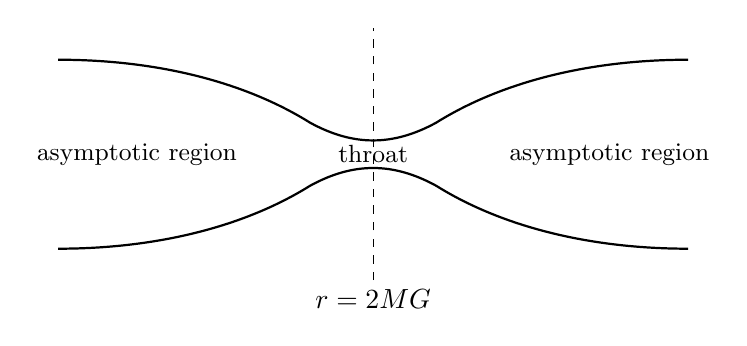
\begin{tikzpicture}[scale=1.0]
\draw[thick] (-4,1.2)
.. controls (-2.7,1.2) and (-1.6,0.9) .. (-0.8,0.4)
.. controls (-0.25,0.1) and (0.25,0.1) .. (0.8,0.4)
.. controls (1.6,0.9) and (2.7,1.2) .. (4,1.2);

\draw[thick] (-4,-1.2)
.. controls (-2.7,-1.2) and (-1.6,-0.9) .. (-0.8,-0.4)
.. controls (-0.25,-0.1) and (0.25,-0.1) .. (0.8,-0.4)
.. controls (1.6,-0.9) and (2.7,-1.2) .. (4,-1.2);

\draw[dashed] (0,-1.6) -- (0,1.6);
\node[below] at (0,-1.6) {$r=2MG$};
\node at (0,0) {\small throat};
\node at (-3.0,0) {\small asymptotic region};
\node at (3.0,0) {\small asymptotic region};
\end{tikzpicture}
\caption{Схематическое пространственное сечение расширенной геометрии Шварцшильда. Это осторожная реконструкция данного в лекции изображения моста, а не буквальный расчёт вложения.}
\end{figure}

Теперь следует поправка. Это сечение наводит на мысль о мосте между двумя асимптотическими областями и потому соблазняет думать, что можно попасть из одной вселенной в другую, пройдя через горловину. Лекция сначала позволяет такому предположению возникнуть, а затем причинно его опровергает. Чтобы перейти из одной внешней области в другую, мировая линия должна была бы где-то на диаграмме Пенроуза стать более пологой, чем нулевая линия под углом \(45^\circ\). Это запрещено. Следовательно, мост Эйнштейна--Розена непроходим.

Лектор также подчёркивает, почему пространственная картина может вводить в заблуждение. Это картина \emph{пространства в один момент времени}; но причинного времени для прохождения попросту недостаточно. Можно, вольно выражаясь, сказать, что мост открывается и закрывается прежде, чем что-либо успеет его пересечь. Ещё лучше просто снова посмотреть на диаграмму Пенроуза и непосредственно считать с неё причинный ответ.

\section{Построение реальной чёрной дыры из падающей внутрь нулевой оболочки}

На этом этапе лекция полностью меняет задачу. Мы больше не считываем свойства вечной чёрной дыры. Мы строим реальную чёрную дыру.

Модель выбрана из соображений простоты. Мы рассматриваем не коллапсирующую звезду со сложной внутренней структурой, а тонкую сферическую оболочку падающего излучения. Это световая оболочка, и потому она движется внутрь со скоростью света. При достаточно малом радиусе энергия на этой оболочке концентрируется достаточно сильно, чтобы образовалась чёрная дыра.

Второй ингредиент — теорема об оболочке в её общей релятивистской форме.

\paragraph{Замечание.} Для сферически-симметричной оболочки, используемой в этой лекции, внутренняя область представляет собой плоское пространство-время, тогда как внешняя область описывается геометрией Шварцшильда. Это рабочая формулировка теоремы об оболочке, или утверждение типа Биркгофа, на которое опирается лекция. Здесь она не доказывается.

Лектор мотивирует это, сначала напоминая ньютонову теорему об оболочке: внутри сферической оболочки гравитационного поля нет, тогда как вне оболочки поле такое же, как у точечной массы в центре. Затем он формулирует соответствующую релятивистскую версию в единственной форме, нужной здесь: внутри — плоское пространство-время, снаружи — геометрия Шварцшильда. Оболочка может двигаться; правило остаётся тем же.

Этого достаточно, чтобы построить пространство-время коллапса. Сама оболочка нулевая, поэтому её нужно изобразить под углом \(45^\circ\). По одну сторону этой нулевой линии геометрия плоская. По другую сторону — геометрия Шварцшильда. Правило можно суммировать так:
\begin{equation}
\begin{aligned}
\text{inside shell} &= \text{flat spacetime},\\
\text{outside shell} &= \text{Schwarzschild geometry}.
\end{aligned}
\end{equation}

Тогда правило склейки становится почти смущающе простым:

\begin{enumerate}
\item Нарисуйте диаграмму Пенроуза для плоского пространства-времени и оставьте только область внутри входящей оболочки.
\item Нарисуйте диаграмму Пенроуза для геометрии Шварцшильда и оставьте только область вне той же самой оболочки.
\item Отбросьте неподходящие части.
\item Сшейте две оставшиеся части вдоль траектории оболочки.
\end{enumerate}

Именно так построение и идёт на доске: отбрасывается неподходящая половина одной картины, отбрасывается неподходящая половина другой, а подходящие половины склеиваются вдоль оболочки.

\begin{figure}[htbp]
\centering
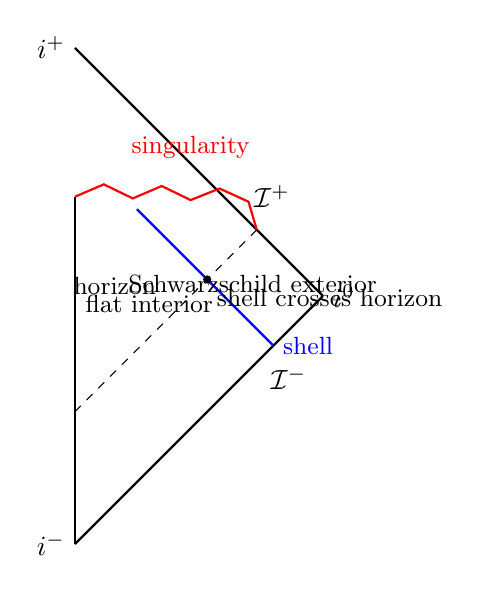
\begin{tikzpicture}[scale=1.05]
\coordinate (im) at (0,-3.0);
\coordinate (ip) at (0,3.0);
\coordinate (i0) at (3.0,0.0);
\coordinate (S)  at (0,1.2);
\coordinate (E)  at (2.2,0.8);
\coordinate (P)  at (2.4,-0.6);
\coordinate (Q)  at (0.75,1.05);
\coordinate (H)  at (0,-1.4);
\coordinate (X)  at (1.6,0.2);

\draw[thick] (im) -- (S);
\draw[thick] (im) -- (i0);
\draw[thick] (ip) -- (i0);

\draw[red,thick] (S) -- (0.35,1.35) -- (0.7,1.18) -- (1.05,1.33) -- (1.4,1.16) -- (1.75,1.30) -- (2.1,1.14) -- (E);
\node[red,above] at (1.4,1.55) {\small singularity};

\draw[thick,blue] (P) -- (Q);
\node[blue,right] at (P) {\small shell};

\draw[dashed] (H) -- (E);
\node[above left] at (1.1,-0.1) {\small horizon};

\filldraw (X) circle (1.2pt);
\node[below right] at (X) {\small shell crosses horizon};

\node at (0.9,-0.1) {\small flat interior};
\node at (2.15,0.15) {\small Schwarzschild exterior};

\node[left] at (im) {$i^-$};
\node[left] at (ip) {$i^+$};
\node[right] at (i0) {$i^0$};
\node[below right] at (2.25,-0.75) {$\mathcal{I}^-$};
\node[above right] at (2.05,0.95) {$\mathcal{I}^+$};
\end{tikzpicture}
\caption{Причинная реконструкция геометрии коллапса. Оболочка — это входящая нулевая линия; с её внутренней стороны сохраняется плоское пространство-время, а с внешней — геометрия Шварцшильда.}
\end{figure}

\begin{figure}[htbp]
\centering
\includegraphics[width=0.76\textwidth]{lecture_08_figure_06.png}
\caption{Завершённое построение на доске после того, как плоская внутренняя область и шварцшильдовская внешняя область были склеены вдоль синей падающей оболочки. Пунктирная линия \(45^\circ\) проводится назад от будущей конечной точки сингулярности, чтобы определить положение горизонта событий.}
\lectureframe{00:57:30}
\end{figure}

Сама оболочка не испытывает ничего особенного в тот момент, когда она просто переходит из плоской части диаграммы в шварцшильдовскую. Это светоподобная оболочка, и она продолжает двигаться внутрь, пока не достигнет сингулярности. Существенная структура определяется не локальной драмой на оболочке, а причинной организацией склеенного пространства-времени.

\begin{classroomqa}
\audiencequestion{Есть ли разрыв, когда коллапсирующая оболочка пересекает свой шварцшильдовский радиус?}
\lecturerresponse{Нет. При этом пересечении локально сингулярного ничего не происходит. Оболочка продолжает двигаться по своей нулевой траектории. Особенность этого события причинная: после того как оболочка пересекла свой радиус \(2MG\), никакой направленный в будущее путь не может вернуть её на бесконечность.
\lecturetimestamp{00:56:19--00:56:42}}
\end{classroomqa}

\section{Горизонт до прихода: загадка горизонта событий}

Теперь наступает концептуальная кульминация лекции. После того как пространство-время коллапса построено, естественно возникает вопрос: где находится горизонт? Или, как выражается лектор, где находится точка невозврата?

\paragraph{Определение.} Горизонт событий — это граница между теми событиями, которые ещё могут послать направленный в будущее причинный сигнал в \(\mathcal{I}^+\), и теми, которые не могут.

На лекции его находят по диаграмме. Начните в углу, где сингулярность встречается с будущей светоподобной бесконечностью, и проследите назад светоподобную линию под углом \(45^\circ\). Эта прослеженная назад светоподобная линия и есть горизонт событий.

Но затем лектор настаивает на втором пункте, и именно он тревожит студентов. Горизонт не просто появляется в тот момент, когда оболочка пересекает свой собственный радиус Шварцшильда, и затем остаётся на месте. На увеличенном рисунке на доске горизонт начинается как крошечная захваченная область вблизи центра, расширяется наружу через часть пространства-времени, которая всё ещё плоская, и лишь позже встречается с падающей оболочкой. В событии этой встречи оболочка пересекает свой собственный радиус Шварцшильда. Выше этого события горизонт является обычным горизонтом постоянного радиуса у полностью сформировавшейся чёрной дыры.

\begin{figure}[htbp]
\centering
\resizebox{0.96\linewidth}{!}{%
\begin{tikzpicture}[scale=1.08,>=Latex]
\coordinate (im) at (0,-3.0);
\coordinate (ip) at (0,3.0);
\coordinate (i0) at (3.0,0.0);
\coordinate (S)  at (0,1.2);
\coordinate (E)  at (2.2,0.8);
\coordinate (P)  at (2.4,-0.6);
\coordinate (Q)  at (0.75,1.05);
\coordinate (H)  at (0,-1.4);
\coordinate (X)  at (1.6,0.2);

\draw[thick] (im) -- (S);
\draw[thick] (im) -- (i0);
\draw[thick] (ip) -- (i0);

\draw[red,thick] (S) -- (0.35,1.35) -- (0.7,1.18) -- (1.05,1.33) -- (1.4,1.16) -- (1.75,1.30) -- (2.1,1.14) -- (E);
\node[red,above left] at (S) {\small singularity};

\draw[very thick,red] (H) -- (E);

\draw[thick,blue] (P) -- (Q);

\filldraw (X) circle (1.2pt);

\draw[gray] (0.0,-2.1) .. controls (0.85,-1.95) and (1.9,-1.3) .. (2.8,-0.2);
\draw[gray] (0.0,-1.2) .. controls (0.95,-1.0) and (1.8,-0.45) .. (2.45,0.35);
\draw[gray] (0.0,-0.2) .. controls (0.8,-0.05) and (1.45,0.35) .. (1.95,0.95);

\node[below right] at (2.28,-0.72) {$\mathcal{I}^-$};
\node[above right] at (2.12,0.92) {$\mathcal{I}^+$};

\draw[very thick,red] (3.2,-1.15) -- (3.75,-1.15);
\node[anchor=west] at (3.85,-1.15) {\small event horizon};
\draw[thick,blue] (3.2,-1.55) -- (3.75,-1.55);
\node[anchor=west] at (3.85,-1.55) {\small infalling shell};
\filldraw (3.48,-1.95) circle (1.2pt);
\node[anchor=west] at (3.85,-1.95)
  {\small shell reaches \(r=2MG\)};
\end{tikzpicture}
}
\caption{Диаграмма коллапса с выделенным горизонтом событий, прослеженным назад. Часть горизонта лежит в области, которая всё ещё локально плоская и до которой оболочка ещё не дошла.}
\end{figure}

Именно на этом поразительном эффекте сосредоточена остальная часть лекции. Часть горизонта лежит в плоском пространстве-времени. Оболочка туда ещё не пришла, и её даже нельзя увидеть на прошлом световом конусе наблюдателя. Наблюдатель не ощущает никакого гравитационного поля и тем не менее не может выбраться. Причина не в локальной силе, а в глобальном причинном будущем данного события.

\begin{classroomqa}
\audiencequestion{Означает ли эта конструкция, что нельзя пересечь оболочку,
или что нельзя пересечь горизонт? Где находится оболочка, когда её горизонт всё
ещё лежит внутри неё?}
\lecturerresponse{Оболочку можно пересечь. Горизонт — это другая светоподобная
поверхность: это граница между событиями, которые могут причинно связаться с
\(\mathcal I^+\), и событиями, которые не могут. Падающая оболочка встречает эту
границу ровно тогда, когда пересекает радиус Шварцшильда, соответствующий
её полной энергии. До встречи часть горизонта событий проходит через
плоскую внутреннюю область; после встречи оболочка оказывается внутри
сформировавшейся чёрной дыры.
\lecturetimestamp{00:58:42--01:01:06}}
\end{classroomqa}

\begin{classroomqa}
\audiencequestion{Если внутренняя область плоская, а оболочка всё ещё далеко,
почему человек, находящийся чуть внутри горизонта, не может пересечь его до
прихода оболочки?}
\lecturerresponse{Нарисуйте максимально быструю возможную мировую линию
наружу — \(45^\circ\) световой луч. Даже такой луч, выпущенный из события
внутри прослеженного назад горизонта, встречает падающую оболочку слишком
поздно и оканчивается на сингулярности. Ходьба ещё медленнее. Фраза
\emph{оболочка ещё не пересекла} неполна, пока не выбрана
временная координата; причинная диаграмма даёт ответ, не зависящий от
координат. Приходящее космическое микроволновое фоновое излучение —
не тот же самый пример, потому что оно не является коллапсирующей
сферической оболочкой, создающей эту геометрию.
\lecturetimestamp{01:01:07--01:04:03}}
\end{classroomqa}

\section{Зеркала и попытки изменить будущее}

Теперь вопросы превращают диаграмму в лабораторию. Предположим, что падающую световую оболочку можно отразить прежде, чем она окажется захваченной. Тогда изменится предполагаемая история коллапса, а вместе с ней и горизонт событий. Это не противоречие: горизонт событий определяется только после того, как задана полная история пространства-времени.

\begin{classroomqa}
\audiencequestion{Что, если прямо снаружи предполагаемого радиуса
Шварцшильда поместить идеально отражающее зеркало, чтобы оболочка
отскочила обратно наружу?}
\lecturerresponse{В этой идеализированной истории падающая светоподобная
линия поворачивает наружу у зеркала и достигает будущей границы; чёрная
дыра на исходной диаграмме не образуется. По-настоящему невесомое зеркало
невозможно, и физическое зеркало само вносит вклад в тензор
энергии-импульса, но мысленный эксперимент проясняет логический момент:
только после того, как оболочка пересекает действительный горизонт
событий, выбраться наружу уже невозможно.
\lecturetimestamp{01:04:33--01:05:54}}
\end{classroomqa}

\begin{classroomqa}
\audiencequestion{Может ли наблюдатель, знающий, что оболочка приближается,
быстро отправить зеркало или сигнал, чтобы заставить её развернуться?}
\lecturerresponse{Только если необходимую аппаратуру можно достаточно рано
разместить вне горизонта. Алиса может заранее устроить так, чтобы Боб послал
оболочку, и поэтому может знать, что приближается, ещё до того, как это увидит.
Однако как только её событие оказывается внутри горизонта, ни зеркало, ни
инструкция уже не могут вовремя достичь нужной внешней точки. Знание о
будущем эксперименте не открывает причинного пути, который запрещён
диаграммой.
\lecturetimestamp{01:05:55--01:08:18}}
\end{classroomqa}

\begin{classroomqa}
\audiencequestion{Что происходит с зеркалом, уже находящимся внутри горизонта, и
находится ли сингулярность бесконечно далеко в его будущем?}
\lecturerresponse{Зеркало — просто ещё один обречённый объект. Оно может
локально отражать свет, но отражённый свет, зеркало и Алиса все оканчиваются на
сингулярности. Типичная падающая мировая линия достигает её за конечное
собственное время. Бесконечно далёк только идеальный верхний угол
компактифицированной диаграммы. Попытка оставаться вблизи этого угла
потребовала бы неограниченно больших ускорения и энергии; кроме того,
между фиксированными событиями ускоренные часы накапливают меньше
собственного времени, чем инерциальные, а не больше.
\lecturetimestamp{01:08:19--01:10:19}}
\end{classroomqa}

\begin{classroomqa}
\audiencequestion{Если коллапсирующая оболочка огромна, может ли кто-то внутри
оболочки, но далеко от её будущего центра, просто оставаться там, пока она
проходит мимо?}
\lecturerresponse{Да, при условии, что событие этого человека всё ещё находится вне
горизонта событий. Находиться внутри материальной оболочки — не то же самое,
что находиться внутри чёрной дыры. Излучение может ударить по наблюдателю и
причинить ему вред, но это локальное взаимодействие с оболочкой и оно отлично от
причинного вопроса о возможности выбраться.
\lecturetimestamp{01:10:21--01:11:24}}
\end{classroomqa}

\section{Временные срезы и растущий горизонт}

Под \emph{моментом времени} в искривлённом пространстве-времени понимается выбранная пространственноподобная гиперповерхность. Семейство таких поверхностей образует слоение, а приписывание каждой поверхности числа задаёт временную координату. Разные слоения по-разному разрезают одну и ту же диаграмму коллапса. Они по-разному определяют, какие удалённые события одновременны, но не меняют того, какие светоподобные лучи достигают бесконечности.

\begin{figure}[htbp]
\centering
\includegraphics[width=0.77\textwidth]{lecture_08_figure_07.png}
\caption{Поздний рисунок на доске с несколькими зелёными
пространственноподобными срезами. Эти срезы задают временную координату; чёрные
светоподобные границы и их причинные отношения от этого выбора не зависят.}
\lectureframe{01:17:30}
\end{figure}

\begin{classroomqa}
\audiencequestion{Можно ли переформулировать эту загадку, сравнив в один момент
расстояние от наблюдателя до горизонта с расстоянием от горизонта
до оболочки?}
\lecturerresponse{Это может давать полезную интуицию после выбора слоения,
но выражение \emph{в один момент} зависит от координат. Чистая
конструкция состоит в том, чтобы провести семейство пространственноподобных срезов.
Ранние срезы пересекают большую оболочку, но не содержат захваченной центральной
области; более поздние пересекают растущий горизонт внутри всё ещё падающей оболочки;
один выделенный срез проходит через событие, в котором оболочка пересекает свой собственный
радиус Шварцшильда.
\lecturetimestamp{01:11:26--01:14:21}}
\end{classroomqa}

\begin{classroomqa}
\audiencequestion{Растёт ли радиус Шварцшильда по мере того, как горизонт
раскрывается наружу, и почему горизонт продолжает расти после того, как оболочка
пересекает его?}
\lecturerresponse{Конечный радиус Шварцшильда \(2MG\) фиксирован, потому что
фиксирована полная масса \(M\). То, что растёт на ранних пространственноподобных срезах, — это
ареальный радиус сечения горизонта. Он начинается в центре,
увеличивается, пока не встречает оболочку при \(r=2MG\), а затем перестаёт расти. Выше
события встречи горизонт является линией постоянного \(r\), а именно \(r=2MG\), хотя
компактификация не делает эту линию ни вертикальной на вид, ни однородной в
метрическом отношении.
\lecturetimestamp{01:14:22--01:16:15}}
\end{classroomqa}

\begin{classroomqa}
\audiencequestion{Что происходит с наблюдателем, который первоначально находится на половине конечного
радиуса Шварцшильда? Не должен ли такой наблюдатель почувствовать гравитацию только тогда, когда
прибудет оболочка?}
\lecturerresponse{Именно так. Наблюдатель сначала пересекает растущий горизонт
событий, всё ещё находясь в плоском пространстве-времени, и не ощущает никакой внезапной силы. Падающая
оболочка излучения — физический объект и позже может стать ощутимой; горизонт событий
— нет. Его пересечение означает лишь, что всякий направленный в будущее причинный путь теперь
не достигает бесконечности. В этом точном смысле горизонт призрачен.
\lecturetimestamp{01:16:17--01:17:45}}
\end{classroomqa}

\begin{classroomqa}
\audiencequestion{Может ли наблюдатель, начавший достаточно рано, двигаться наружу быстрее растущего горизонта и выбраться?}
\lecturerresponse{Да. У событий вне горизонта есть исходящие причинные пути к \(\mathcal I^+\); у событий внутри их нет. На выбранном срезе можно сравнить имеющееся радиальное расстояние со временем, остающимся до того, как входящая оболочка перекроет путь, но точный критерий дают нулевые линии. Ни один наблюдатель не видит, как наружу стремительно движется материальный горизонт, потому что нет локальной поверхности, которую можно было бы увидеть.
\lecturetimestamp{01:17:46--01:18:54}}
\end{classroomqa}

\section{Что сохраняет диаграмма}

Фигуры на странице не следует воспринимать как изображение в масштабе. Небольшой уголок может представлять бесконечную область пространства-времени, тогда как большой участок — небольшой физический интервал. Компактификация намеренно жертвует метрическими размерами, чтобы сохранить нулевые направления. Сохраняются причинно-следственные отношения: кто кому может послать сигнал, какие события могут влиять на какие другие события и какие мировые линии оказываются в ловушке из-за ограничения скорости света.

\begin{classroomqa}
\audiencequestion{Если рисунок настолько сильно искажает длины и времена, что же он тогда отображает верно?}
\lecturerresponse{Он отображает световые лучи и, следовательно, причинную структуру. Чтобы найти горизонт событий, проследите обратно от будущей бесконечности последний исходящий нулевой луч. Пытаться вывести ответ из кажущихся расстояний на странице ненадёжно. После того как причинная диаграмма построена, вопросы о сигналах, о том, можно ли выбраться, и о том, откуда возврата нет, имеют геометрические ответы, хотя метрический масштаб опущен.
\lecturetimestamp{01:18:56--01:21:45}}
\end{classroomqa}

\begin{classroomqa}
\audiencequestion{Сколько времени требуется, чтобы освоиться с диаграммами Пенроуза настолько, чтобы пользоваться ими интуитивно?}
\lecturerresponse{Недолго. Практический рецепт состоит в том, чтобы рисовать их, прослеживать нулевые линии и проверять возможные мировые линии, пока причинные ограничения не станут привычными. Интуиция здесь приобретается работой с диаграммами, а не догадками без них.
\lecturetimestamp{01:21:49--01:22:05}}
\end{classroomqa}

\begin{classroomqa}
\audiencequestion{Является ли этот наглядный метод противоположностью тому, что бывает в квантовой механике, где математика часто надёжнее, чем наглядное представление?}
\lecturerresponse{В значительной степени — да. Общая теория относительности — классическая физика. Четырёхмерное искривлённое пространство-время трудно буквально представить, и диаграмма Пенроуза всё ещё абстрактна, но причинную геометрию такого пространства-времени можно изобразить и исследовать гораздо дальше, чем это возможно для лежащей в основе квантовой механики реальности. Это различие — часть того, что делает эти диаграммы столь мощными.
\lecturetimestamp{01:22:05--01:22:58}}
\end{classroomqa}